\documentclass[letterpaper,12pt]{article}
\usepackage{amsmath}  % improve math presentation
\usepackage{graphicx} % takes care of graphic including machinery
\usepackage{mathrsfs}


\usepackage[final]{hyperref} % adds hyper links inside the generated pdf file
\hypersetup{
	colorlinks=true,       % false: boxed links; true: colored links
	linkcolor=blue,        % color of internal links
	citecolor=blue,        % color of links to bibliography
	filecolor=magenta,     % color of file links
	urlcolor=blue         
}

\title{Sixth Assignment for Computational Physics}
\date{\today}
\author{Xinyu Liu}


\begin{document}
\maketitle
\tableofcontents

\newpage

\section{My Github Page URL}
\url{https://github.com/rising1227/phys-ga2000}

\section{PCA analysis of a real astrophysical data set}

The Associated Code for this assignment is ps6.py.

\subsection{A}

We've imported the data with astropy package. As a physicist, we know that hydrogen atoms have typical energy level structure with $hc/\lambda = 13.6eV*(1/n^2 - 1/m^2)$. For the related optical frequency in observed data set, we take n = 2 and m = 3,4,5. The transition wavelength should be 656.47nm, 486.27nm and 434.17nm. We plotted several flux data for different galaxy and also plotted some vertical line related to the special transition wavelength. We do observe some kind of structure around those wavelength.

\begin{table}[!h]
    \centering
    \caption{Flux wrt wavelength for galaxy 1}
    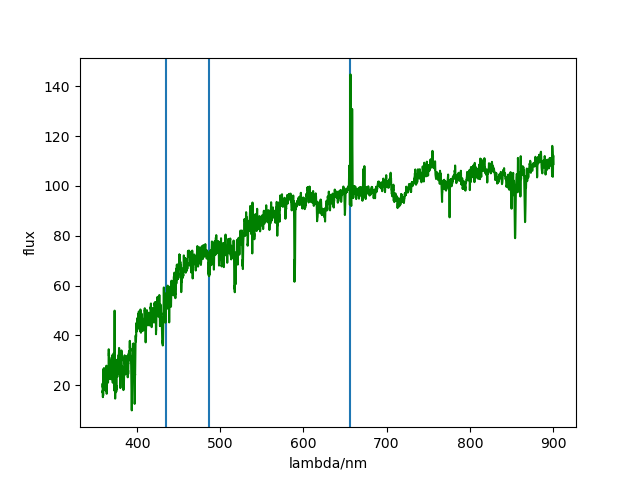
\includegraphics[width=11cm]{7-1-0.png}
\end{table}%

\begin{table}[!h]
    \centering
    \caption{Flux wrt wavelength for galaxy 2}
    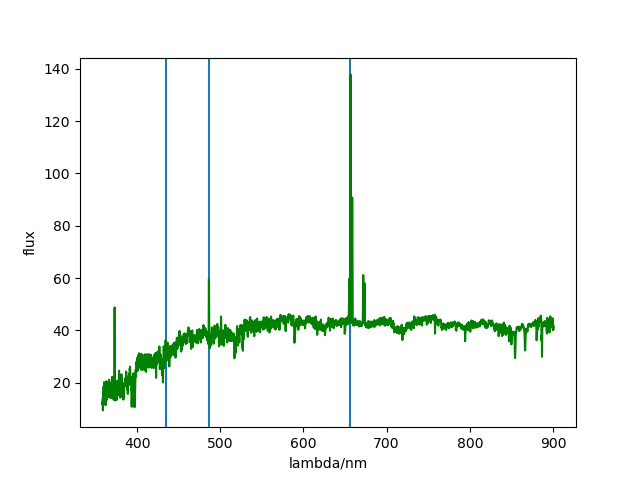
\includegraphics[width=11cm]{7-1-1.png}
\end{table}%

\begin{table}[!h]
    \centering
    \caption{Flux wrt wavelength for galaxy 3}
    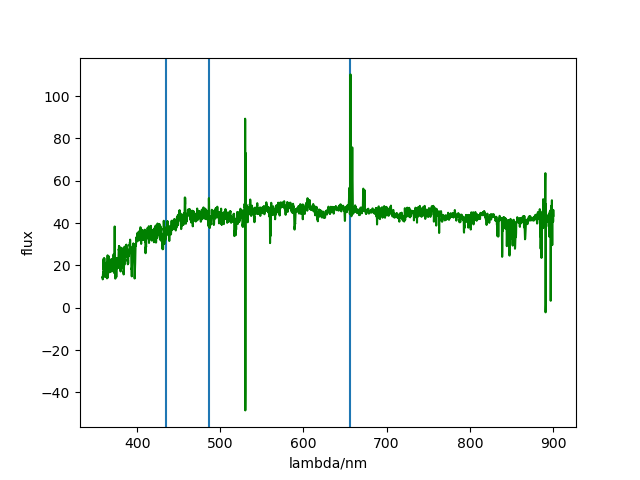
\includegraphics[width=11cm]{7-1-2.png}
\end{table}%

\begin{table}[!h]
    \centering
    \caption{Flux wrt wavelength for galaxy 4}
    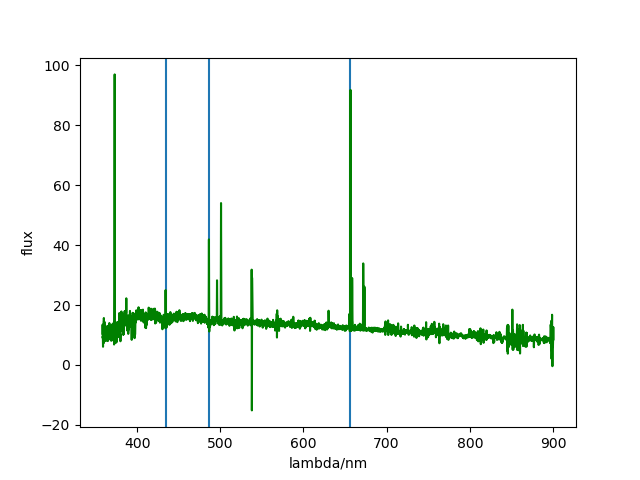
\includegraphics[width=11cm]{7-1-3.png}
\end{table}%

\begin{table}[!h]
    \centering
    \caption{Flux wrt wavelength for galaxy 5}
    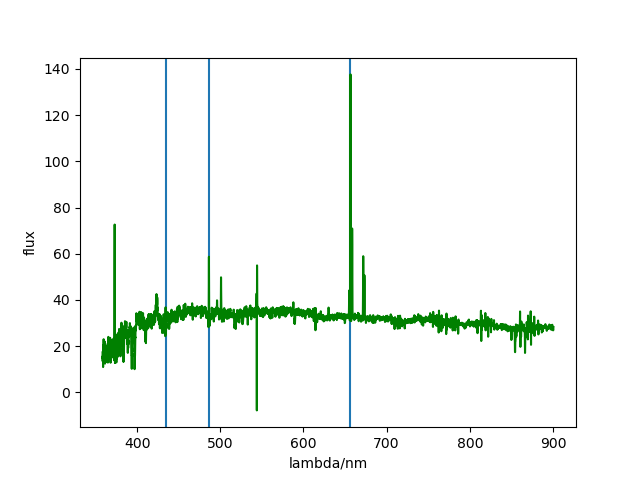
\includegraphics[width=11cm]{7-1-4.png}
\end{table}%
\newpage

\subsection{B,C}

We've finished the required normalization process in our code. The result is stored in a Array Normalization and Res for future use.

\subsection{D}

We measure the covariance matrice and carried out the PCA. We plotted five engenstate with largest eigenvalue.

\begin{table}[!h]
    \centering
    \caption{1st PCA eigenstate}
    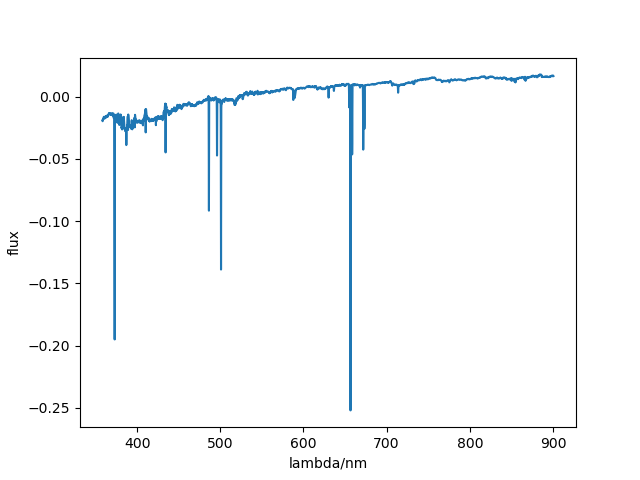
\includegraphics[width=11cm]{7-4-0.png}
\end{table}%

\begin{table}[!h]
    \centering
    \caption{2nd PCA eigenstate}
    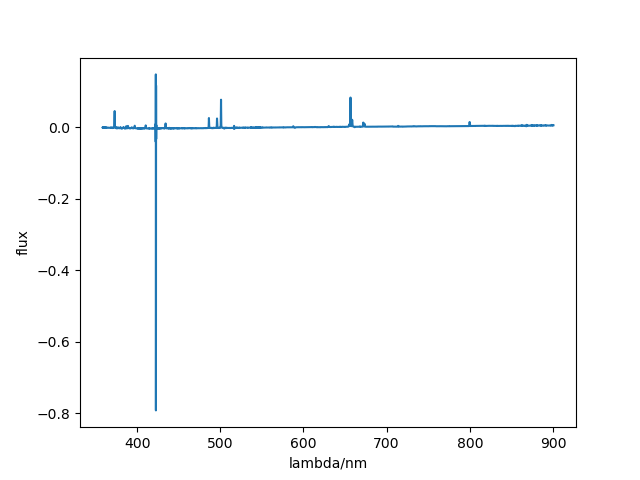
\includegraphics[width=11cm]{7-4-1.png}
\end{table}%

\begin{table}[!h]
    \centering
    \caption{3rd PCA eigenstate}
    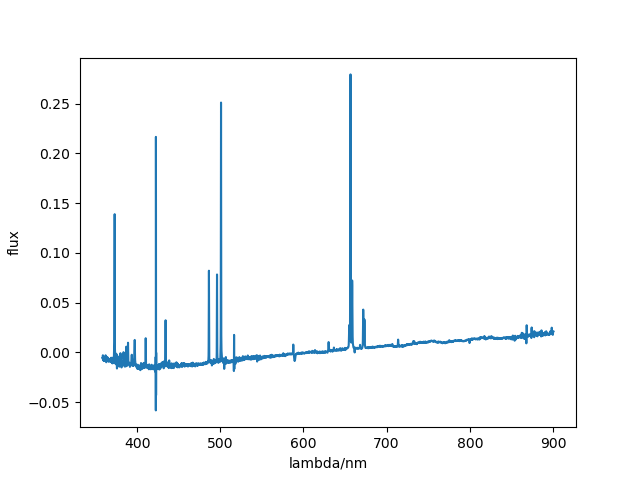
\includegraphics[width=11cm]{7-4-2.png}
\end{table}%

\begin{table}[!h]
    \centering
    \caption{4th PCA eigenstate}
    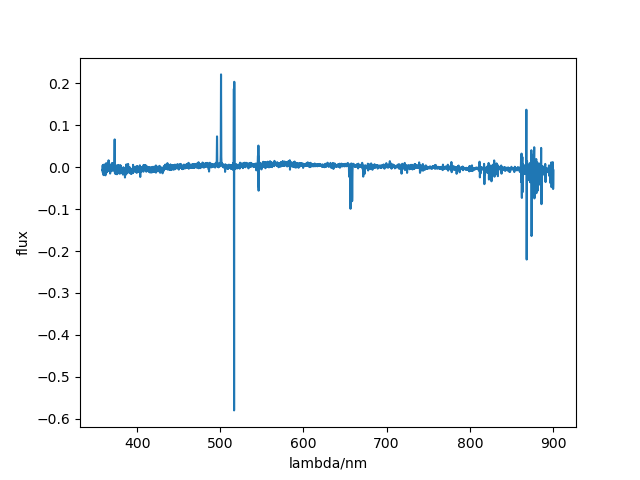
\includegraphics[width=11cm]{7-4-3.png}
\end{table}%

\begin{table}[!h]
    \centering
    \caption{5th PCA eigenstate}
    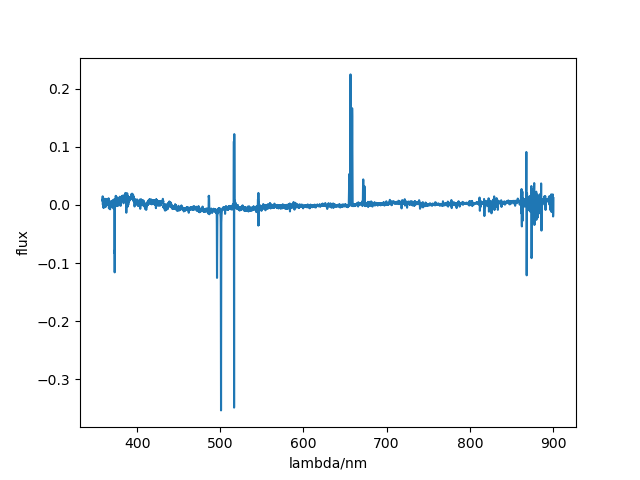
\includegraphics[width=11cm]{7-4-4.png}
\end{table}%
\newpage

\subsection{E}

We can similarly calculate the eigenstate by doing SVD directly to R matrice. We've explicitly test that the eigenstate by SVD is equvalent to what's found before(we've calculated the cosine of related angle of two states.)

We found that the SVD method cost 37.32s while diagonialize a $R^TR$ matrice in PCA cost 25.4s. It seems that doing SVD cost slightly more time.

\subsection{F}

We also found that the conditional number for doing a diagonalization for $R^TR$ is much larger than doing SVD to R(which is very easy to understand, since SVD is somehow a squareroot of diagonalization). The conditional number for SVD is 5205738 while for PCA diagonalization is 27099608379355. When the data set is even larger, doing SVD, although cannot make computation faster, do enhance the stablization of the computation.

\subsection{G}

We can explicitly calculate the coefficient on first 5 eigenstates by doing rotation. Then we can approximate the real data by only storing several coeffieicnt before those 5 eigenstates. We've plotted the approximated data and real flux data in the following diagram:

\begin{table}[!h]
    \centering
    \caption{flux 0 vs approximation}
    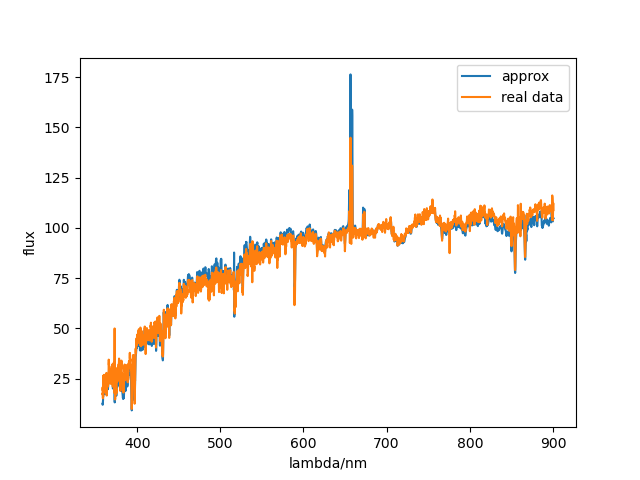
\includegraphics[width=11cm]{7-7-0.png}
\end{table}%

\begin{table}[!h]
    \centering
    \caption{flux 1 vs approximation}
    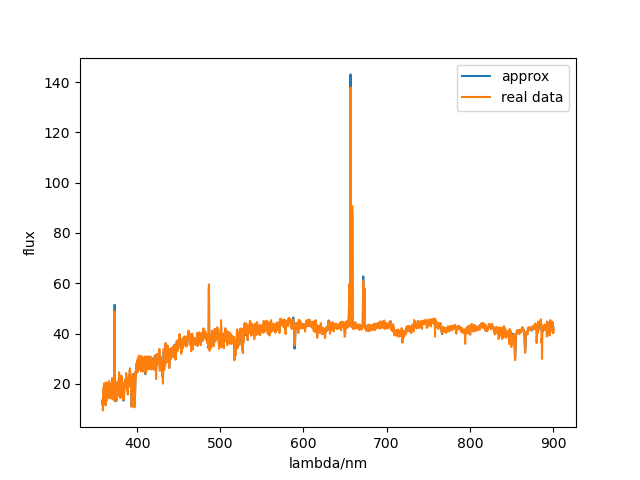
\includegraphics[width=11cm]{7-7-1.png}
\end{table}%

\begin{table}[!h]
    \centering
    \caption{flux 2 vs approximation}
    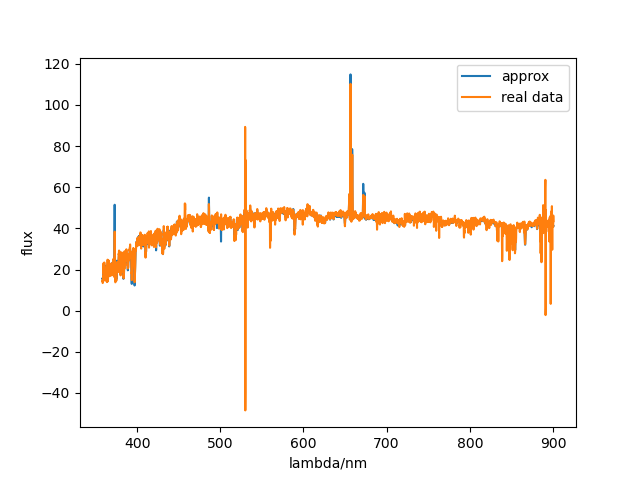
\includegraphics[width=11cm]{7-7-2.png}
\end{table}%

\begin{table}[!h]
    \centering
    \caption{flux 3 vs approximation}
    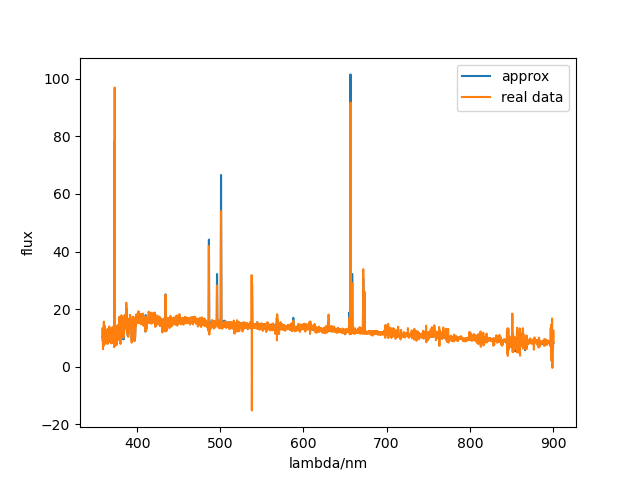
\includegraphics[width=11cm]{7-7-3.png}
\end{table}%

\begin{table}[!h]
    \centering
    \caption{flux 4 vs approximation}
    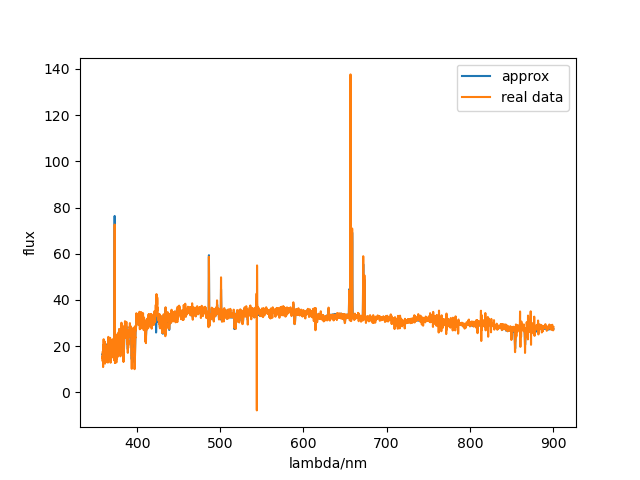
\includegraphics[width=11cm]{7-7-4.png}
\end{table}%

\newpage



\subsection{H}

We've plotted C0 vs C1 and C1 vs C2:

\begin{table}[!h]
    \centering
    \caption{C0 vs C1}
    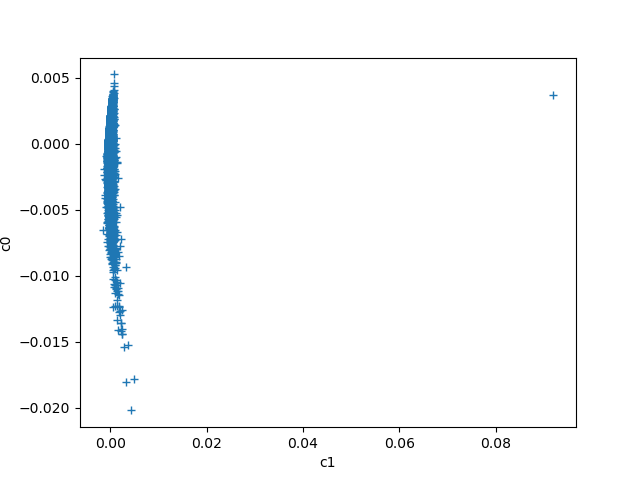
\includegraphics[width=11cm]{7-8-1.png}
\end{table}%

\begin{table}[!h]
    \centering
    \caption{C1 vs C2}
    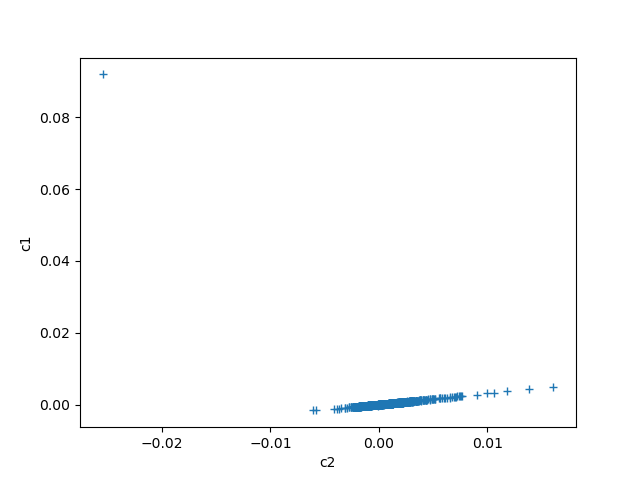
\includegraphics[width=11cm]{7-8-2.png}
\end{table}%

\newpage

\subsection{I}

We've calculated the Error of approximation with different number of principal components from 0 to 20. Here's our result and we've explicitly found that the error goes down when Nc grows higher. When Nc equals 20 the error(sum of the square of difference between real data and approximation) goes down to 8675.

\begin{table}[!h]
    \centering
    \caption{5th PCA eigenstate}
    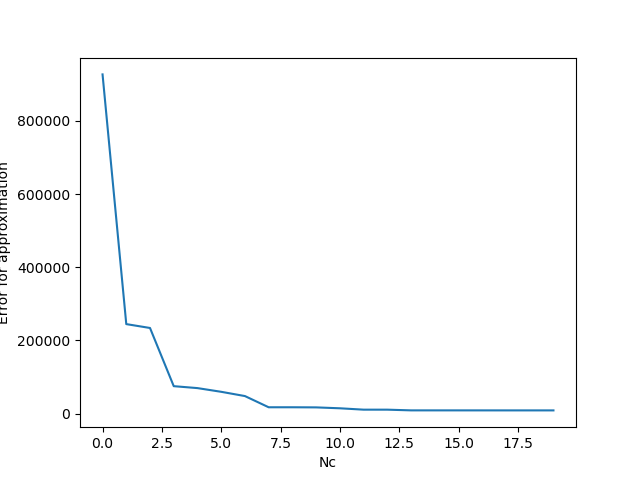
\includegraphics[width=11cm]{7-9.png}
\end{table}%


\end{document}